\documentclass{beamer}
\usepackage[english, russian]{babel}
\usepackage[T2A]{fontenc}
\usepackage[utf8]{inputenc}
\usepackage{indentfirst}
\usepackage{amsmath, amsfonts, amssymb, amsthm, mathtools}
\usepackage[export]{adjustbox}
\usepackage{graphicx} 
\graphicspath{ {./images/} }

\usepackage{subcaption}
\usepackage{verbatim}

\usepackage{minted}{\setlength{\parskip}{0pt}}

\usepackage{hyperref}

\hypersetup{
    colorlinks=true,
    linkcolor=blue,
    filecolor=magenta,      
    urlcolor=black,
    pdftitle={Overleaf Example},
    pdfpagemode=FullScreen,
    }


\title{Лабораторная работа № 14. \\ Настройка файловых служб Samba}
\author{Данила Стариков \\ НПИбд-02-22}
\institute{Российский университет дружбы народов имени Патриса Лумумбы}
\date{2024}

\begin{document}

\frame{\titlepage}

\begin{frame}
\frametitle{Цель работы}
\begin{itemize}
    \item Приобретение навыков настройки доступа групп пользователей к общим ресурсам по протоколу SMB.
\end{itemize}
\end{frame}

\begin{frame}
\frametitle{Настройка сервера Samba}
    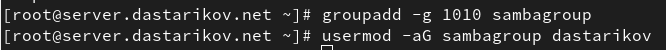
\includegraphics[width=0.8\textwidth]{../images/image01.png}
    \captionof{figure}{Создание группы sambagroup и добавления в нее пользователя dastarikov.}
\end{frame}


\begin{frame}
\frametitle{Настройка сервера Samba}
    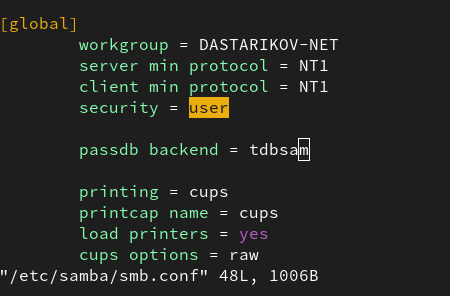
\includegraphics[width=0.8\textwidth]{../images/image27.png}
    \captionof{figure}{Изменение конфигурации samba на сервере.}
\end{frame}


\begin{frame}
\frametitle{Настройка сервера Samba}
    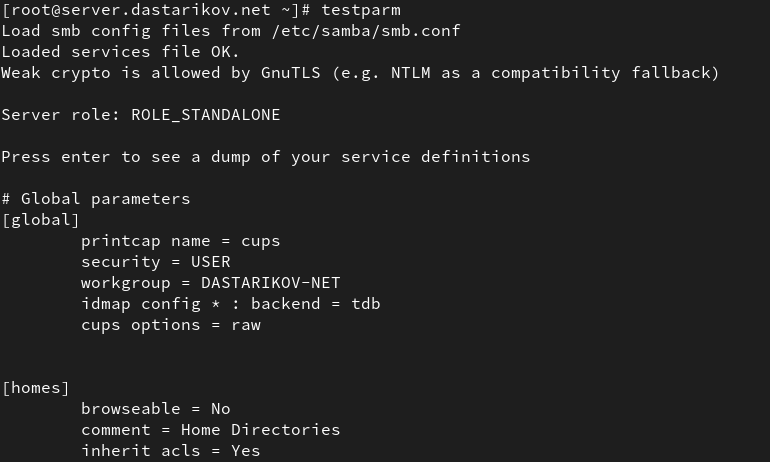
\includegraphics[width=0.8\textwidth]{../images/image02.png}
    \captionof{figure}{Проверка правильности синтаксиса файла samba.conf.}
\end{frame}


\begin{frame}
\frametitle{Настройка сервера Samba}
    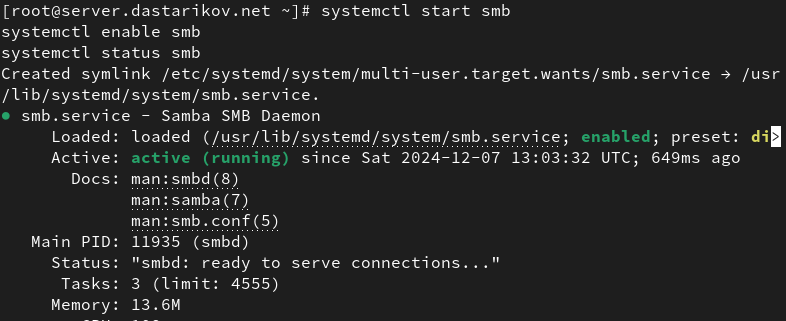
\includegraphics[width=0.8\textwidth]{../images/image03.png}
    \captionof{figure}{Включение демона Samba.}
\end{frame}


\begin{frame}
\frametitle{Настройка сервера Samba}
    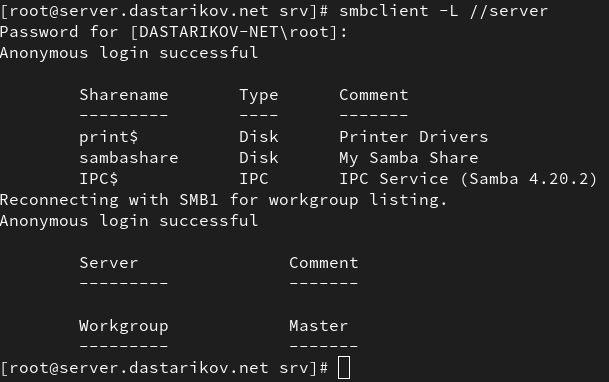
\includegraphics[width=0.8\textwidth]{../images/image16.png}
    \captionof{figure}{Проверка наличия общего доступа к серверу.}
\end{frame}


\begin{frame}
\frametitle{Настройка сервера Samba}
    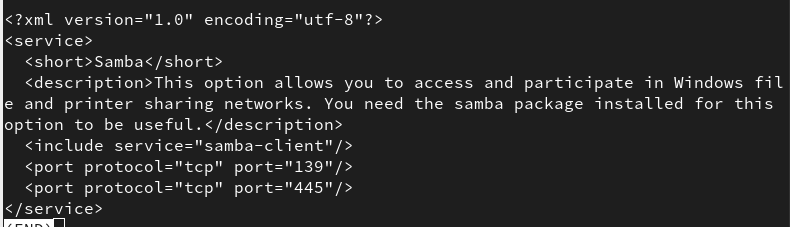
\includegraphics[width=0.8\textwidth]{../images/image04.png}
    \captionof{figure}{Просмотр конфигурации межсетевого экрана Samba.}
\end{frame}


\begin{frame}
\frametitle{Настройка сервера Samba}
    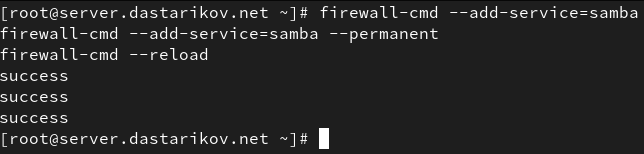
\includegraphics[width=0.8\textwidth]{../images/image05.png}
    \captionof{figure}{Настройка межсетевого экрана.}
\end{frame}


\begin{frame}
\frametitle{Настройка сервера Samba}
    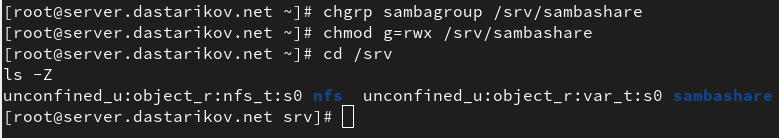
\includegraphics[width=0.8\textwidth]{../images/image06.png}
    \captionof{figure}{Настройка прав доступа для каталога с разделяемым ресурсом sambashare.}
\end{frame}


\begin{frame}
\frametitle{Настройка сервера Samba}
    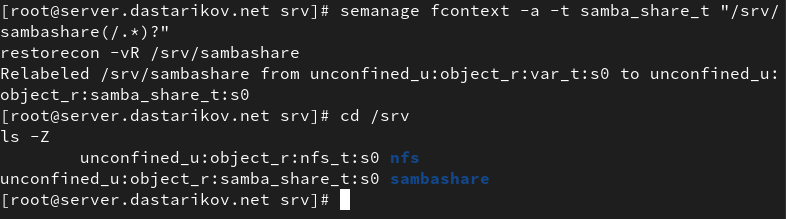
\includegraphics[width=0.8\textwidth]{../images/image08.png}
    \captionof{figure}{Настройка SELinux для каталога с разделяемым ресурсом smbshare.}
\end{frame}


\begin{frame}
\frametitle{Настройка сервера Samba}
    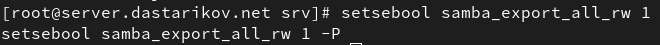
\includegraphics[width=0.8\textwidth]{../images/image09.png}
    \captionof{figure}{Настройка разрешений через флаги SELinux.}
\end{frame}


\begin{frame}
\frametitle{Настройка сервера Samba}
    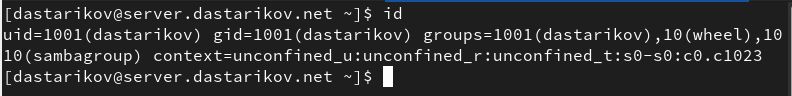
\includegraphics[width=0.8\textwidth]{../images/image10.png}
    \captionof{figure}{Просмотр групп пользователя dastarikov.}
\end{frame}


\begin{frame}
\frametitle{Настройка сервера Samba}
    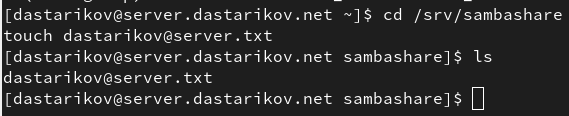
\includegraphics[width=0.8\textwidth]{../images/image11.png}
    \captionof{figure}{Создание файла на разделяемой ресурсе.}
\end{frame}


\begin{frame}
\frametitle{Настройка сервера Samba}
    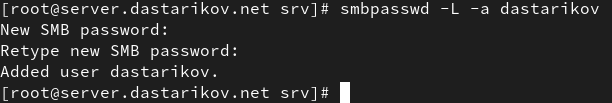
\includegraphics[width=0.8\textwidth]{../images/image12.png}
    \captionof{figure}{Добавление dastarikov в базу пользователей Samba.}
\end{frame}


\begin{frame}
\frametitle{Монтирование файловой системы Samba на клиенте}
    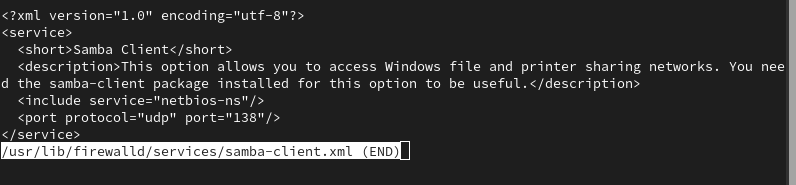
\includegraphics[width=0.8\textwidth]{../images/image13.png}
    \captionof{figure}{Просмотр конфигурации межсетевого экрана для клиента Samba.}
\end{frame}


\begin{frame}
\frametitle{Монтирование файловой системы Samba на клиенте}
    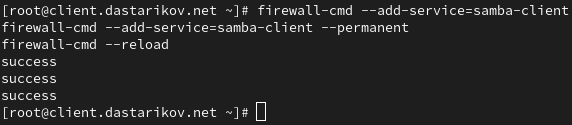
\includegraphics[width=0.8\textwidth]{../images/image14.png}
    \captionof{figure}{Настройка межсетевого экрана клиента.}
\end{frame}


\begin{frame}
\frametitle{Монтирование файловой системы Samba на клиенте}
    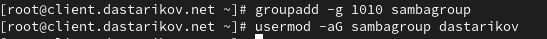
\includegraphics[width=0.8\textwidth]{../images/image15.png}
    \captionof{figure}{Создание аналогичной группы на клиенте и добавления в нее dastarikov.}
\end{frame}


\begin{frame}
\frametitle{Монтирование файловой системы Samba на клиенте}
    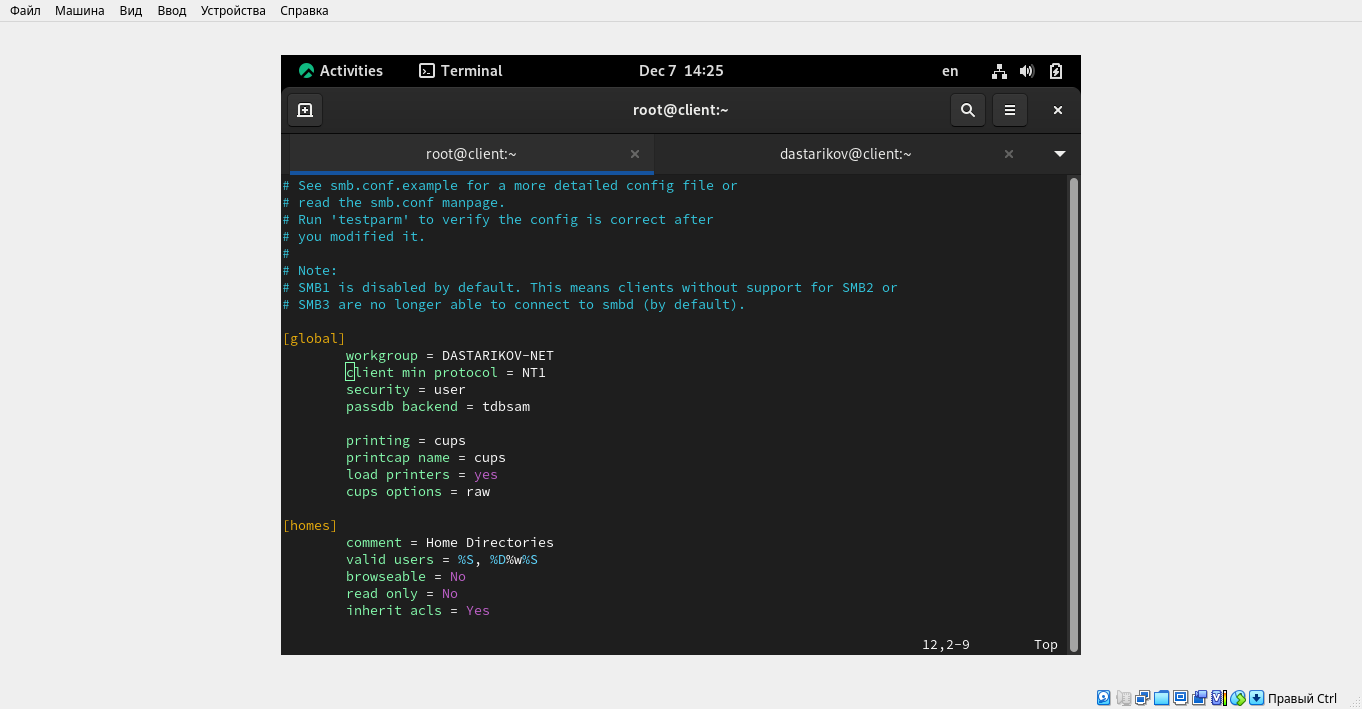
\includegraphics[width=0.8\textwidth]{../images/image17.png}
    \captionof{figure}{Изменение конфигурации samba на клиенте.}
\end{frame}


\begin{frame}
\frametitle{Монтирование файловой системы Samba на клиенте}
    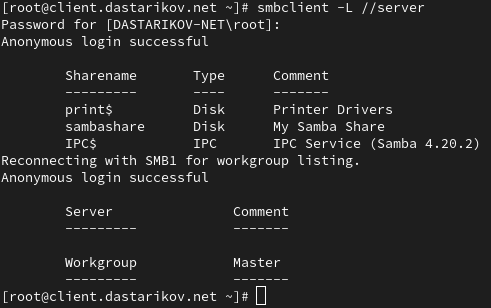
\includegraphics[width=0.8\textwidth]{../images/image18.png}
    \captionof{figure}{Подключение к серверу под пользователем root.}
\end{frame}


\begin{frame}
\frametitle{Монтирование файловой системы Samba на клиенте}
    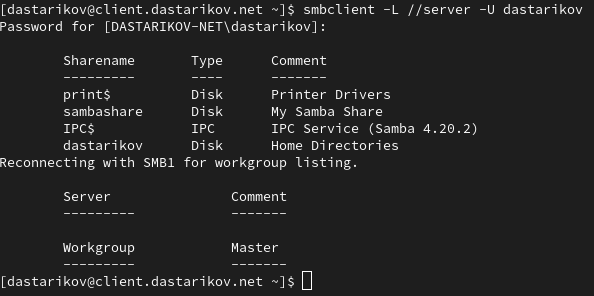
\includegraphics[width=0.8\textwidth]{../images/image19.png}
    \captionof{figure}{Подключение к серверу под пользователем dastarikov.}
\end{frame}


\begin{frame}
\frametitle{Монтирование файловой системы Samba на клиенте}
    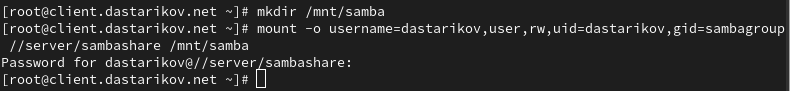
\includegraphics[width=0.8\textwidth]{../images/image20.png}
    \captionof{figure}{Монтирование разделяемого ресурса на клиенте.}
\end{frame}


\begin{frame}
\frametitle{Монтирование файловой системы Samba на клиенте}
    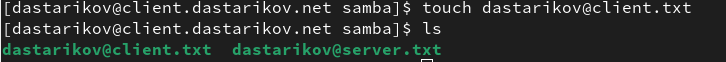
\includegraphics[width=0.8\textwidth]{../images/image21.png}
    \captionof{figure}{Проверка возможности создавать файлы на разделяемом ресурсе.}
\end{frame}


\begin{frame}
\frametitle{Монтирование файловой системы Samba на клиенте}
    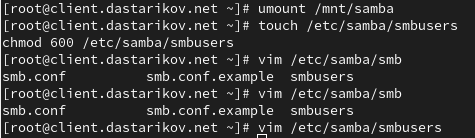
\includegraphics[width=0.8\textwidth]{../images/image22.png}
    \captionof{figure}{Отмонтирование каталога samba и создание файла smbusers.}
\end{frame}


\begin{frame}
\frametitle{Монтирование файловой системы Samba на клиенте}
    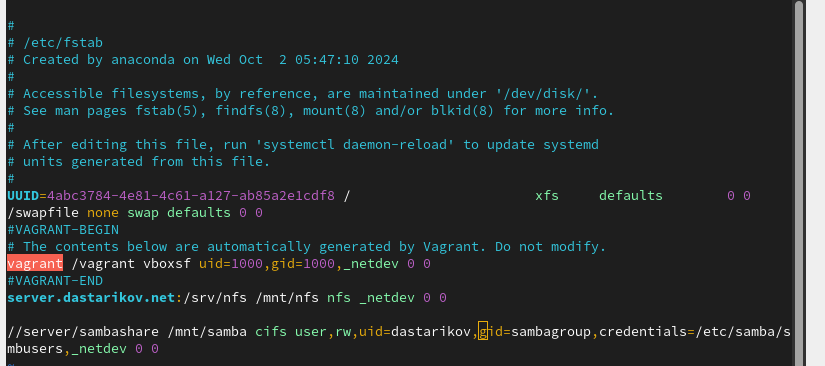
\includegraphics[width=0.8\textwidth]{../images/image23.png}
    \captionof{figure}{Изменение файла /etc/fstab.}
\end{frame}


\begin{frame}
\frametitle{Монтирование файловой системы Samba на клиенте}
    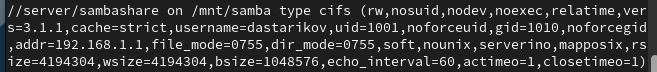
\includegraphics[width=0.8\textwidth]{../images/image24.png}
    \captionof{figure}{Настройка автоматического монтирования каталога для разделяемых ресурсов.}
\end{frame}


\begin{frame}
\frametitle{Внесение изменений в настройки внутреннего окружения виртуальных машин}
    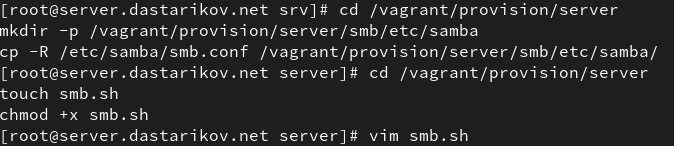
\includegraphics[width=0.8\textwidth]{../images/image25.png}
    \captionof{figure}{Изменение настроек внутреннего окружения на виртуальной машине server.}
\end{frame}


\begin{frame}
\frametitle{Внесение изменений в настройки внутреннего окружения виртуальных машин}
    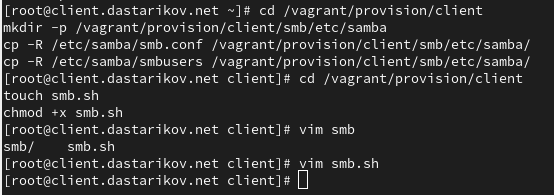
\includegraphics[width=0.8\textwidth]{../images/image26.png}
    \captionof{figure}{Изменение настроек внутреннего окружения на виртуальной машине client.}
\end{frame}

\begin{frame}
\frametitle{Выводы}
\begin{itemize}
    \item В результате лабораторной работы познакомились с настройкой доступа групп пользователей к общим ресурсам по протоколу SMB.
\end{itemize}
\end{frame}
\end{document}
